\documentclass[12pt, a4paper]{report}
\usepackage[utf8x]{inputenc}
\usepackage{ragged2e}
\usepackage{pdflscape}
\usepackage{graphicx}
\graphicspath{ {./images/} }
\usepackage{geometry}
\renewcommand{\contentsname}{İçindekiler Tablosu}
\usepackage[ddmmyyyy]{datetime}
\renewcommand{\dateseparator}{.}
\renewcommand{\figurename}{Şekil}
\renewcommand{\bibname}{Referanslar}
\geometry{
	top=2.5cm,
	left=2.5cm,
	right=2.5cm,
	bottom=2.5cm
}
% Title Page
\title{TRAFİKTE YORGUNLUK TESPİT SİSTEMİ TASARIM DOKÜMANI}
\author{Sema YEŞİLKAYA}
\renewcommand{\thesection}{\arabic{section}.}
\begin{document}
\maketitle
\tableofcontents{} \newpage
\section{Giriş}
 \pagenumbering{arabic} 
Yorgunluk, sürücülerin tepki sürelerini yavaşlatan ve karar verme yeteneklerini olumsuz etkileyen kritik bir faktördür. Bu durum, özellikle uzun mesafe sürüşlerinde ve gece saatlerinde artan bir risk oluşturur. Geliştirilecek sistem, sürücünün yorgunluk seviyesini gerçek zamanlı olarak izleyerek potansiyel tehlikeleri önceden tespit etmeyi ve uygun uyarılar sağlamayı amaçlamaktadır. Bu sayede, sürücülerin dinlenmeye ihtiyaç duydukları zamanlarda bilgilendirilmesi ve olası kazaların önlenmesi hedeflenmektedir.

Projede kullanılacak yapay zeka teknikleri, sürücünün yüzündeki mikro ifadeleri, göz kırpma sıklığını ve baş hareketlerini analiz edebilecek gelişmiş görüntü işleme algoritmalarını içermektedir. Ayrıca, kalp atış hızı gibi fizyolojik veriler, zaman serisi analizi yoluyla incelenecek ve yorgunluk seviyesinin belirlenmesinde kullanılacaktır. 
\begin{figure}[!h]
	\centering
	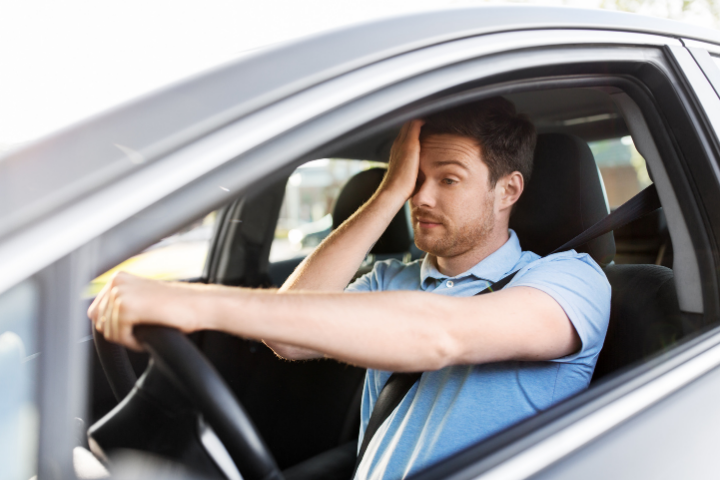
\includegraphics[width=17cm, height=6cm, keepaspectratio]{yorgunluk.png}
	\caption{Yorgun sürücü}
\end{figure}
\section{Literatür Araştırması}
Literatür araştırması bölümünde, yorgunluk tespiti ve trafik güvenliği alanında yapılmış önceki çalışmalar incelenmektedir. Bu çalışmalar, yorgunluk algılama tekniklerinin gelişimini, kullanılan sensör teknolojilerini ve algoritmaları kapsamaktadır. Ayrıca, bu teknolojilerin trafik kazalarını azaltmadaki etkinliği ve sürücü davranışları üzerindeki etkileri de değerlendirilmektedir.\cite{vural2018gercek}'de yer alan Karolinska Uykululuk Skalası ibaresi üzerine bu skala araştırılmış olup sürücüler üzerinde analiz edilmesi gereken veriler buradan belirlenmek üzere karar alınmıştır. Projemiz, mevcut sistemlerin sınırlılıklarını ele almakta ve yorgunluk tespitinde yapay zeka ve makine öğrenimi tekniklerinin entegrasyonu ile daha etkili çözümler sunmayı hedeflemektedir.\newpage

	\begin{landscape}
		\section{Süreç Planlaması}
	\begin{figure}[!htbp] %[h]
		\centering
		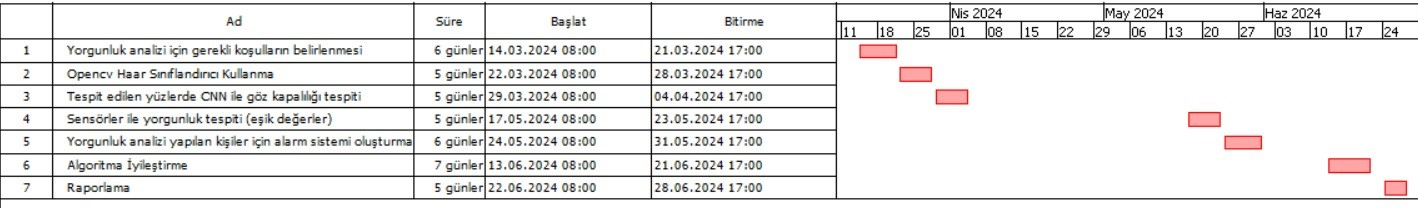
\includegraphics[height=7cm, width=27cm]{gantt.jpg}
		%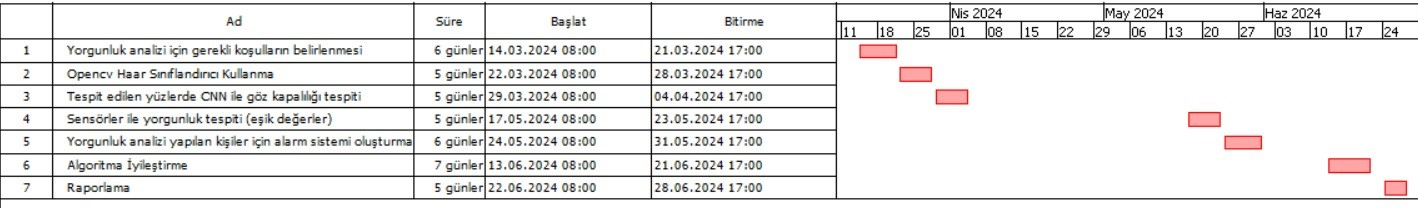
\includegraphics[angle=90, width=\textwidth]{gantt.jpg}
		\caption{Gantt Chart}		   	
		\label{gantt}
	\end{figure}
	Şekil \ref{gantt}'de görülebileceği üzere
	iş akış planı gösterilmektedir.
\end{landscape}
\pagebreak 
\section{Metodoloji}
Projede, araç içindeki sürücülerin yorgunluk seviyelerini belirlemek için gelişmiş yapay zeka ve makine öğrenimi teknikleri kullanılacaktır. Yorgunluk tespiti için, farklı sensörlerden alınan veriler üzerinde görüntü işleme, zaman serisi analizi ve davranışsal örüntü tanıma gibi yöntemlerin uygulanması düşülmektedir.
Sürücünün yüzünün önünde, sürücünün yüzünü algılayan ve derin öğrenmeyi kullanarak sürücünün gözlerini kapalı veya açık olarak tanımlayan bir kamera, bu veri sistemi yardımıyla sürücünün uyuşukluğunu tespit eder.\par
 Haar Cascade, bir görüntü veya videodaki nesneleri tanımlamak için kullanılan ve özellik kavramına dayanan bir makine öğrenimi nesne algılama algoritmasıdır.\par
  Haar Cascade sınıflandırıcı, Haar Cascade sınıflandırıcı yüz algılama için kullanılır ve ardından görüntüden yüzü çıkarır. Görüntüden yüz çıkarıldıktan sonra, bu görüntüyü, yüzün görüntüsündeki gözlerin kapalı veya açık olduğunu sınıflandıran CNN sınıflandırıcısını eğitmek için kullanacağım.

\subsection{Görüntü İşleme}
Görüntü işleme teknikleri, sürücünün yüzünden yorgunluk belirtilerini tespit etmek için kullanılacaktır. Bu teknikler, sürücünün göz kırpma sıklığını, göz kapaklarının pozisyonunu, esneme sıklığını ve başın pozisyonunu analiz eder. Görüntü işleme algoritmaları, sürücünün yüzündeki değişiklikleri zaman içinde izleyerek yorgunluk belirtilerini saptayabilmektedir.

\subsection{Zaman Serisi Analizi}
Zaman serisi analizi, sürücünün fizyolojik verilerinin zaman içindeki değişimlerini analiz etmek için kullanılacaktır. Kalp atış hızı gibi veriler, yorgunluk seviyesinin bir göstergesi olarak değerlendirilecektir. Bu analiz, yorgunluk seviyelerindeki değişimleri belirlemek için uzun süreli veri akışlarını inceleyecektir.

\subsection{Davranışsal Örüntü Tanıma}
Davranışsal örüntü tanıma, sürücünün davranışsal verilerini analiz ederek yorgunluk belirtilerini tespit etmek için kullanılacaktır. Direksiyon hareketleri, pedal kullanımı ve vites değiştirme gibi sürüş davranışları, yorgunluk seviyesinin belirlenmesinde önemli faktörlerdir. Bu teknik, sürücünün davranışsal verilerini analiz ederek yorgunlukla ilişkili davranışsal değişiklikleri saptayabilir.

Bu tekniklerin kombinasyonu, yorgunluk tespiti için güçlü ve güvenilir bir sistem oluşturacaktır. Sensörlerden elde edilen veriler, bu tekniklerle işlendikten sonra, makine öğrenimi algoritmaları ile eğitilecek ve sürücünün yorgunluk seviyesi sınıflandırılacaktır.

\section{Veri Tabanı ve Veriler}
Sensörler aracılığıyla, sürücünün fizyolojik ve davranışsal verileri toplanacaktır. Karolinska Uykululuk Skalası öncelikle tespit edilmiş olup temelde bu skala ele alınarak veriler analiz edilecektir. Bu veriler; göz hareketleri, yüz ifadeleri, baş hareketleri, kalp atış hızı ve cilt iletkenliği gibi biyometrik ölçümleri içerebilir. Sensör olarak Arduino UNO kullanacağım.
Göz kapalılığı ve açıklığı üzerine \cite{aayushrai_driver_safety}'de bulunan veri setini kullanacağım. Bu veri setinde insanların yorgunluk durumuna göre göz kapaklarının durumu analiz ediliyor. Aynı zamanda \cite{csafak2022derin} çalışmasında kullanılan birçok veri setinden biri de bu ve başarı yüzdesi de yüksek oranda.

\begin{figure}[!htbp] %[h]
	\centering
	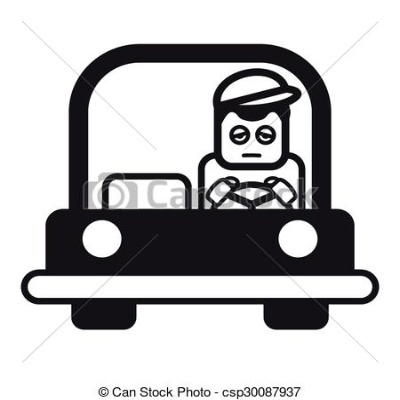
\includegraphics[width=\textwidth]{s1.jpg}
	%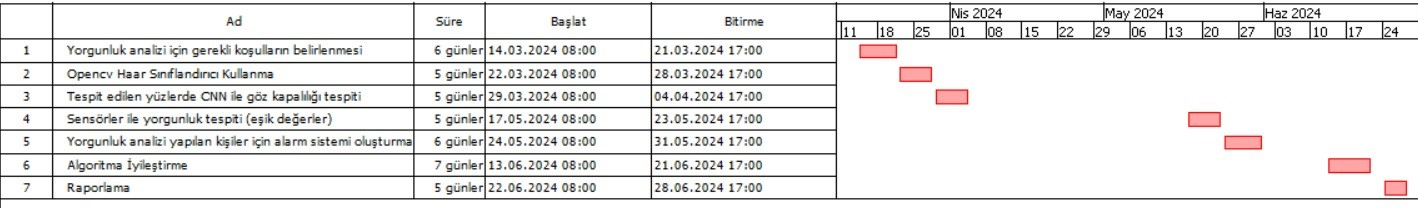
\includegraphics[angle=90, width=\textwidth]{gantt.jpg}
	\caption{Veri setinden örnek.}		   	
	\label{gantt}
\end{figure}
Şekil \ref{gantt}'de görülebileceği üzere
iş akış planı gösterilmektedir.
\maketitle
\subsection{Veri İşleme ve Özellik Çıkarımı}
Veri tabanı için Kaggle başta olmak üzere birçok siteden veri seti taraması yapılacaktır. Bu tarama sonucunda uygun veri setleri dahilinde toplanan veriler, ön işlemeden geçirilecek ve yorgunluk tespiti için gerekli özellikler çıkarılacaktır. Görüntü işleme teknikleri ile sürücünün yüzündeki yorgunluk belirtileri tespit edilecek, fizyolojik değişimler izlenecek ve davranışsal örüntüler analiz edilecektir.
\section{Beklenen Sonuçlar}
Araç içindeki sürücülerin ve yolcuların yorgunluk seviyelerinin doğru bir şekilde tespit edilmesi ve trafik güvenliğinin artırılması beklenmektedir. Sistem, gerçek zamanlı uyarılar sağlayarak sürücülerin ve yolcuların güvenliğini artırmayı hedeflemektedir.
Tespit edilen yorgun sürücülere alarm yöntemleriyle uyarı vermek ve gerekirse aracı uygun bir yere çekmelerini sağlamak gibi bir sonuç sağlamak.

\bibliographystyle{ieeetr}
\bibliography{ref.bib}
%\cite{aayushrai_driver_safety} \cite{akgun2020surucunun} \cite{csafak2022derin} \cite{liu2022review} \cite{rogado2009driver} \cite{sikander2018driver} \cite{zhao2020driver} 
%dosya oluştururken report seçtim bu sebeple atıfta bulunmadan kaynakça yeri oluşmadı ve refences yeri de çıkmadı bibliography olarak oluştu.

\end{document}          
